\documentclass[conference]{IEEEtran}
\IEEEoverridecommandlockouts

\usepackage{cite}
\usepackage{amsmath,amssymb}
\usepackage{graphicx}
\usepackage{booktabs}
\usepackage{array}
\usepackage{xcolor}
\usepackage{microtype}
\usepackage[hidelinks]{hyperref}
\usepackage{url}

\newcommand{\NRecords}{1050}
\newcommand{\NDocs}{15}
\newcommand{\NFinite}{9}
\newcommand{\NNonconv}{6}
\newcommand{\NCertified}{7}
\newcommand{\LatencyMedian}{1.3}
\newcommand{\LatencyMax}{10.4}
\newcommand{\ThesisLatency}{7.5}
\newcommand{\ThesisFacts}{91}
\newcommand{\ThesisEdges}{73}
\newcommand{\BoundTight}{4}
\newcommand{\BoundOverOne}{3}
\newcommand{\BoundUnder}{0}
\newcommand{\SumA}{21}
\newcommand{\SumB}{14}
\newcommand{\SumC}{17}
\newcommand{\SumCprime}{17}
\newcommand{\SumCdprime}{17}
\newcommand{\SumE}{17}
\newcommand{\NCapC}{6}
\newcommand{\ImageDigest}{93feb7fb6c24}


\newcommand{\cls}[1]{\textsc{#1}}
\newcommand{\tex}[1]{\texttt{\detokenize{#1}}}
\graphicspath{{figures/}}

\begin{document}

\title{AuxFlow: A Static Applicability Test for Fixpoint Convergence\\in Multi-Pass LaTeX Builds}

\author{\IEEEauthorblockN{Upayan Mazumder}
\IEEEauthorblockA{School of Computer Science and Engineering (SCOPE)\\
Vellore Institute of Technology\\
Vellore, Tamil Nadu, India\\
\texttt{upayan.mazumder2024@vitstudent.ac.in}}
\and
\IEEEauthorblockN{Banupriya R}
\IEEEauthorblockA{School of Computer Science and Engineering (SCOPE)\\
Vellore Institute of Technology\\
Vellore, Tamil Nadu, India\\
\texttt{banupriya.r@vit.ac.in}}}

\maketitle

\begin{abstract}
A LaTeX document with cross-references, a table of contents, or a bibliography needs several engine runs.
Each run reads the auxiliary files that the previous run wrote.
Five widely used tools decide when to stop with five different tests, and four of them also cap the run count with a fixed constant.
None of them derives the run count from the source.
This paper describes AuxFlow, a compiler front end and static analyzer for a declared subset of LaTeX.
AuxFlow lowers a document to a graph of auxiliary fact instances with lagged edges.
It finds the facts whose values reach a construct that controls how much content the document generates.
It then classifies the document before any engine run.
We test AuxFlow on \NDocs{} documents, seven stopping strategies, and ten repetitions in a pinned container (\NRecords{} records).
All \NCertified{} documents that AuxFlow certifies receive a bound that is at least the measured run count.
AuxFlow flags all \NNonconv{} non-convergent documents before it starts the engine.
Its analysis takes \LatencyMedian{} ms at the median and \LatencyMax{} ms at most.
We also report a guard that we added after the first measurement.
The guard changed three declared false negatives into UNKNOWN results.
\end{abstract}

\begin{IEEEkeywords}
LaTeX, build systems, static analysis, fixpoint iteration, attribute grammars
\end{IEEEkeywords}

%% ---------------------------------------------------------------------------------------------
\section{Introduction}

LaTeX resolves a cross-reference in two steps.
The first engine run writes the value of each label to an auxiliary file.
The next engine run reads that file and prints the value.
A table of contents, a bibliography, and a list of figures work the same way.
The number of runs that a document needs is therefore a property of its reference structure.

In practice, tools discover this number by running the engine.
\texttt{latexmk} compares checksums of the files that the engine wrote and stops after five repeats by default~\cite{latexmk}.
Tectonic stops after six passes~\cite{tectonic}.
ConTeXt stops after nine.
Typst stops after five layout iterations~\cite{typst}.
Table~\ref{tab:oracles} lists the five tests and their limits.
No tool derives a limit from the document.

Some documents never settle.
Gaspar gave a one-page document whose page reference grows by one on every run~\cite{gaspar2014}.
A loop bounded by the reference emits one more page each time.
When a tool reaches its limit, three of the five tools report no cause.

We ask a narrower question than ``how many runs does this document need?''.
Prior work answers the general question for fixed graphs.
Static pass numbering is Bochmann's~\cite{bochmann1976} and Alblas's~\cite{alblas1981}.
Bounding fixpoint rounds by a graph parameter is Hecht and Ullman's~\cite{hecht1975}.
Splitting a circular dependency graph into strongly connected components is Jones's~\cite{jones1990}.
Our setting differs in one respect.
A document can change its own dependency graph.
A page reference can change the page count, and the page count decides how many page references exist.
The classical theory does not cover that case.

AuxFlow tests whether the classical theory applies to a given document.
The test is conservative and covers a declared subset of LaTeX.
It is a sufficient condition for the finite-height half of the convergence condition of Magnusson and Hedin~\cite{magnusson2007}.
It does not test the monotonicity half.

This paper makes three contributions.
\begin{enumerate}
\item A declared LaTeX subset, an instance-level graph of auxiliary facts with pass-lag edges, and an influence analysis that classifies a document before it runs (Section~\ref{sec:approach}).
\item A measured comparison of five stopping tests and two AuxFlow configurations on a fifteen-document corpus.
The corpus covers nine published non-convergence mechanisms (Section~\ref{sec:eval}).
\item A report of what the analysis cannot see, including a change that we made after the first measurement (Section~\ref{sec:guard}).
\end{enumerate}

We do not claim to have invented static pass numbering, strongly connected component analysis, graph-derived round bounds, or checksum verification.
Section~\ref{sec:related} places each of these in earlier work.

\begin{table}[t]
\caption{Stopping tests and limits in five deployed tools. Values come from manuals and source code (latexmk 4.88).}
\label{tab:oracles}
\centering
\small
\begin{tabular}{@{}p{0.17\columnwidth}p{0.36\columnwidth}p{0.08\columnwidth}p{0.25\columnwidth}@{}}
\toprule
Tool & Test between runs & Limit & Cause on limit \\
\midrule
latexmk & time, size, and MD5 of all files & 5 & none \\
latexrun~\cite{latexrun} & tool inputs unchanged & none$^{a}$ & none \\
Tectonic & file read, then rewritten, in one run & 6 & file name \\
ConTeXt & MD5 of the \texttt{.tuc} file & 9 & none \\
Typst & hash of layout iterations & 5 & spans and value history \\
\bottomrule
\end{tabular}

\smallskip
\footnotesize $^{a}$No limit is documented. Our run stopped after 10 iterations (Section~\ref{sec:external}).
\end{table}

%% ---------------------------------------------------------------------------------------------
\section{Background and Related Work}
\label{sec:related}

\subsection{The auxiliary round trip}

A \tex{\label} command writes a \tex{\newlabel} record to the \texttt{.aux} file.
At \tex{\begin{document}}, the kernel reads the \texttt{.aux} file from the previous run before it opens the file for writing.
A value written in run $p$ is therefore readable first in run $p+1$.
We call this delay the \emph{pass lag}, and it is exactly one.
Bibliography data pass through BibTeX between two engine runs.

\subsection{Multi-pass analysis and circular attributes}

Bochmann decides how many left-to-right passes an attribute grammar needs~\cite{bochmann1976}.
Alblas separates \emph{simple} multi-pass grammars from \emph{pure} ones.
In the pure case every instance of an attribute can take its own pass number~\cite{alblas1981}.
Deciding the pure case is hard, and finding the minimum number of passes is NP-complete~\cite{raiha1981}.
AuxFlow numbers fact instances, so it works in Alblas's pure setting.
It computes a conservative bound and does not claim a minimum.

Farrow gives conditions under which a circular grammar has a well-defined result~\cite{farrow1986}.
Jones evaluates such grammars by splitting the dependency graph into strongly connected components and ordering them topologically~\cite{jones1990}.
Magnusson and Hedin state the convergence condition: the attribute values on a cycle must form a lattice of finite height, and the functions must be monotone.
They also state that their evaluator does not check it~\cite{magnusson2007}.
AuxFlow supplies a domain-specific check for the first half of that condition.

Krishnan and Van Wyk analyze termination for higher-order attribute grammars, where evaluation creates new trees~\cite{krishnan2012,vogt1989}.
Their analysis works on a fixed grammar and uses a term-ordering proof.
AuxFlow works on the fact graph of one document and uses reachability.
We have not read the work of S\"oderberg and Hedin on circular higher-order attributes in full~\cite{soderberg2013}.
We therefore make no claim against it.

\subsection{Bounds on fixpoint rounds, rates, and build systems}

Hecht and Ullman bound the rounds of an iterative data-flow solver by the depth of the flow graph~\cite{hecht1975,kam1976}.
The AuxFlow plan has the same shape: $P$ runs to propagate and one run to confirm.
Lee and Messerschmitt separate nodes with a fixed output rate from nodes whose rate depends on data~\cite{lee1987}.
AuxFlow draws the same line for documents.
A value that changes only \emph{what} the document says is benign.
A value that changes \emph{how much} content the document generates is not.

Mokhov et al.\ separate dependencies that are known statically from dependencies that depend on computed values~\cite{mokhov2018}.
Erdweg et al.\ build LaTeX with a fixpoint cycle handler and conclude that ``soundly detecting dependencies is a lost cause'' for LaTeX, because even parsing is undecidable~\cite{erdweg2015,erdweg2010}.
Our answer is the declared subset.
Any construct outside it becomes an opaque fact, and an opaque fact makes the document UNKNOWN.

M\"adje formalizes document stability as a recurrence, proves it undecidable by Rice's theorem for arbitrary code, and proposes a fixed iteration cap with an error at the guilty call~\cite{madje2022}.
AuxFlow follows the same framing and adds a static decision for a restricted class.

\subsection{Non-convergence mechanisms}

Published sources describe at least nine mechanisms.
Table~\ref{tab:corpus} lists the ones that we model as corpus members.
M1 and M2 are loops and conditionals that depend on a page reference.
M3 to M7 change the typeset extent of a reference, a float, or a note.
M8 is a nondeterministic auxiliary record.
M9 is a false positive of the kernel warning and is not real non-convergence.

%% ---------------------------------------------------------------------------------------------
\section{Approach}
\label{sec:approach}

Figure~\ref{fig:pipeline} shows the pipeline.
Everything up to the build plan runs without a TeX engine.
Only \texttt{auxflow run} starts a subprocess.

\begin{figure*}[t]
\centering
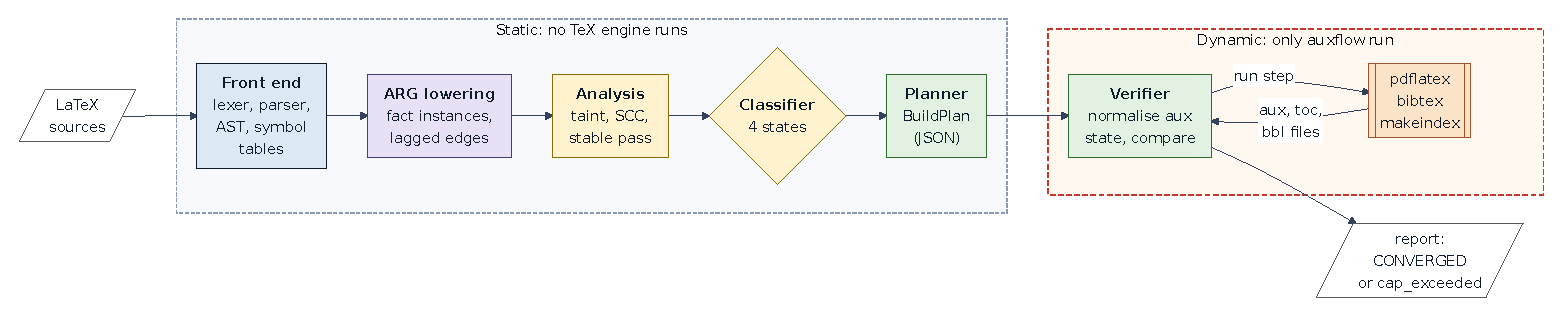
\includegraphics[width=\textwidth]{pipeline.pdf}
\caption{The AuxFlow pipeline. The static stages never start a TeX engine. The verifier is the only stage that does.}
\label{fig:pipeline}
\end{figure*}

\subsection{Declared subset and opaque facts}

The front end has a category-code lexer, a recursive-descent parser, a multi-file syntax tree, and symbol tables for labels, references, citations, packages, files, and counters.
Every node carries a source span.
The subset covers sectioning, labels, references, citations, captions, generated lists, counters, and loops and conditionals over counters.
A small list of packages and commands is inert, because they write no auxiliary state.
Any other command or package becomes an opaque fact.
We do not expand macro bodies.
A local macro is inert only if every command in its body is inert.

\subsection{The Auxiliary Reference Graph}

The Auxiliary Reference Graph (ARG) has one node for each fact \emph{instance}.
An earlier design used one node for each fact \emph{kind}.
That graph is the same eight-node lattice for every document, so analyzing it is a table lookup.
Instance nodes make the problem a real data-flow problem.

Figure~\ref{fig:er} shows the data model.
A fact has a kind (label number, label page, reference use, contents entry, list extent, citation use, bibliography body, counter read, content volume, or opaque), a key, a component, and a source span.
The component is either \texttt{exists} or \texttt{value}.
A dependency edge has a lag and a type.
The types are \cls{aux\_roundtrip}, \cls{tool}, \cls{layout}, and \cls{structural}.
Every edge carries a reason string.
The reason is the text that the diagnostics print.

\begin{figure*}[t]
\centering
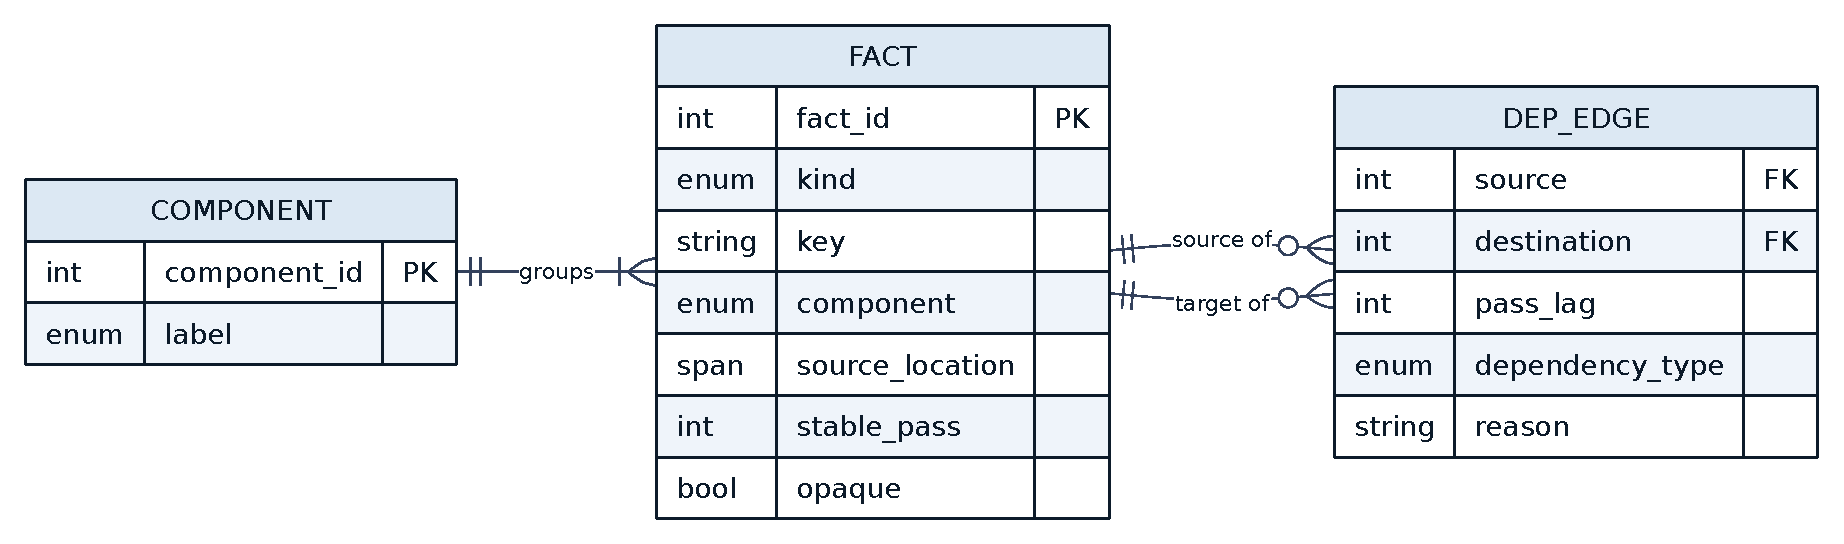
\includegraphics[width=0.78\textwidth]{arg-model.pdf}
\caption{Data model of the ARG. A document lowers to a set of \textsc{fact} and \textsc{dep\_edge} records. Tarjan's algorithm~\cite{tarjan1972} groups facts into components. Each fact keeps its source span, so every diagnostic has a \texttt{file:line:column} location.}
\label{fig:er}
\end{figure*}

\subsection{Stable-pass numbering}

For a fact $f$ with dependencies $\mathrm{deps}(f)$, the stable pass is
\begin{equation}
s(f)=\begin{cases}
1 & \mathrm{deps}(f)=\varnothing,\\
1+\max\limits_{g\in \mathrm{deps}(f)}\bigl(s(g)+\ell(g\!\to\!f)-1\bigr) & \text{otherwise,}
\end{cases}
\label{eq:stable}
\end{equation}
where $\ell$ is the lag of the edge.
Let $P$ be the largest $s(f)$ over the facts that the engine stores in auxiliary files.
The predicted run count is $N=P+1$.
A tool edge counts as lag zero in Eq.~\eqref{eq:stable}, because BibTeX runs between two engine runs.
The numbering follows the longest path on the condensation graph.
It is a bound and not a minimum.

\subsection{Influence analysis}

The ARG joins every generated list to a synthetic \cls{content\_volume} fact that stands for pagination.
The \texttt{exists}/\texttt{value} split removes the edge from a fact's value to pagination.
Without that split, every document with one \tex{\ref} would form a single component, and the analysis would say nothing.

Taint analysis restores the one dependency that matters.
A seed is a fact whose value is read in the bound or condition of a control construct.
A worklist propagates the taint along value edges.
For each tainted fact, the analysis adds a \cls{structural} edge with lag one to \cls{content\_volume}.
The edge carries the source location of the read.
Each fact enters the worklist at most once, so the cost is $O(V+E)$.

An iterative Tarjan algorithm then finds the strongly connected components in $O(V+E)$.
It uses an explicit stack, because a recursive version fails on the larger corpus member.
A non-trivial component has one of three labels.
It is \cls{amplifying} if it contains an internal structural edge.
It is \cls{unknown\_cycle} if it contains an opaque fact.
Otherwise it is \cls{benign}.

The analysis over-approximates.
Taint follows any value edge and does not check that the influence changes a quantity.
A benign document can therefore look amplifying, and the user pays with one flag.
The analysis cannot make the opposite mistake on modeled constructs.
It can, however, miss any feedback that has no seed.

\subsection{Classification and planning}

Figure~\ref{fig:classifier} shows the decision.
The precedence is \cls{amplifying}, then \cls{unknown}, then \cls{benign\_cyclic}, then \cls{certified}.
An amplifying cycle wins over an opaque fact, because it gives the user a more useful report.

\begin{figure*}[t]
\centering
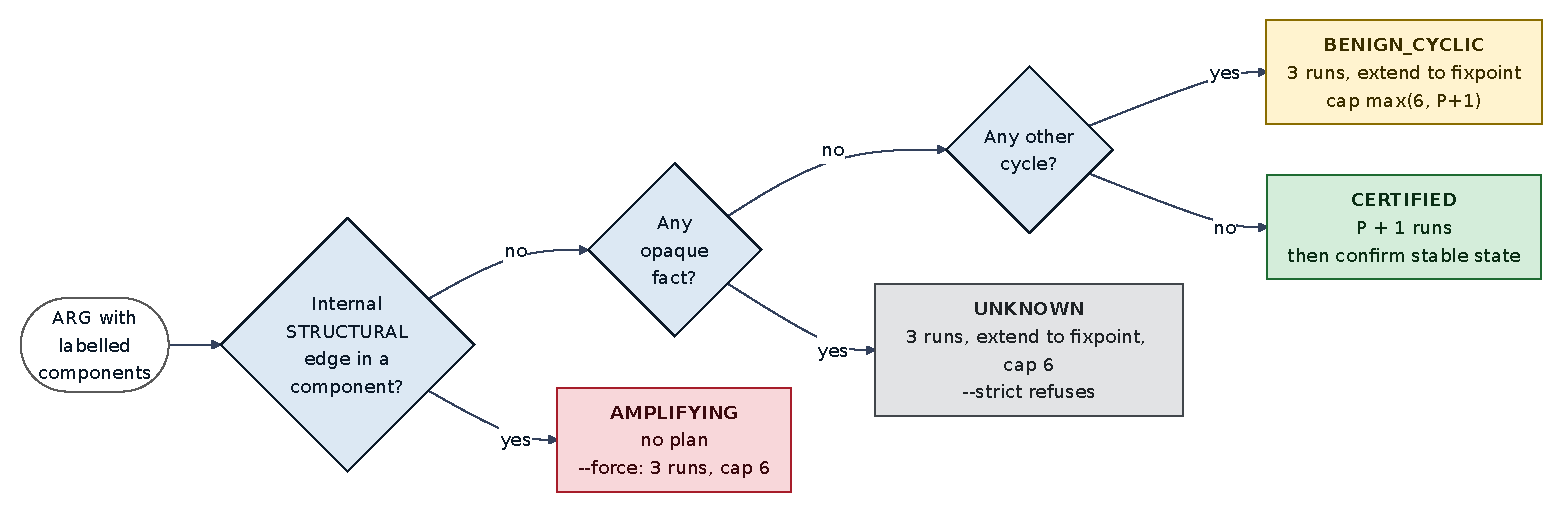
\includegraphics[width=\textwidth]{classifier.pdf}
\caption{Classification and the plan that each state receives. $P$ is the largest stable pass over stored facts. The plan for a non-certified document never has fewer than three engine runs.}
\label{fig:classifier}
\end{figure*}

The planner enforces one safety rule with an assertion.
Only a certified plan uses the derived count.
Every other executable plan has at least three engine runs.
An amplifying document gets no plan unless the user passes \texttt{--force}.
Then the plan has three runs and a cap of six.
The planner also removes work.
It scans only files that the entry file reaches.
It runs BibTeX only if the document has both a citation and a bibliography command.

\subsection{Runtime verification}

Engine warnings are not a sound test.
The kernel warns when a label changed, but base LaTeX gives no warning when a table of contents changed~\cite{rerunfilecheck}.
Active characters in captions cause false warnings~\cite{labelschanged}.
The AuxFlow verifier therefore reads the state directly.

After each engine run, the verifier parses the \texttt{.aux} files, the generated list files, and the bibliography body into a set of canonical records.
It discards order, white space, and the argument-free \tex{\relax} command.
It keeps every unrecognized record, so a changing unknown record cannot look stable.
It compares the set with the set from the previous run.
Figure~\ref{fig:runtime} shows the loop.
If the plan ends and the state still changes, the verifier repeats the last engine step until the state is stable or the cap is reached.
It records a \emph{prediction miss} whenever the observed run count exceeds a certified bound.

Each tool call has a time limit of 600 seconds.
The verifier passes \texttt{-no-shell-escape} to \texttt{pdflatex}.
It rejects auxiliary files that resolve outside the work directory.
AuxFlow does not sandbox TeX, so a user must run only trusted documents.

The verifier is a reimplementation of the checksum approach of \texttt{latexmk}.
We do not claim it as a contribution.
We reimplemented it so that baselines B, C, and E share one normalization and differ only in the stopping test.

\begin{figure*}[t]
\centering
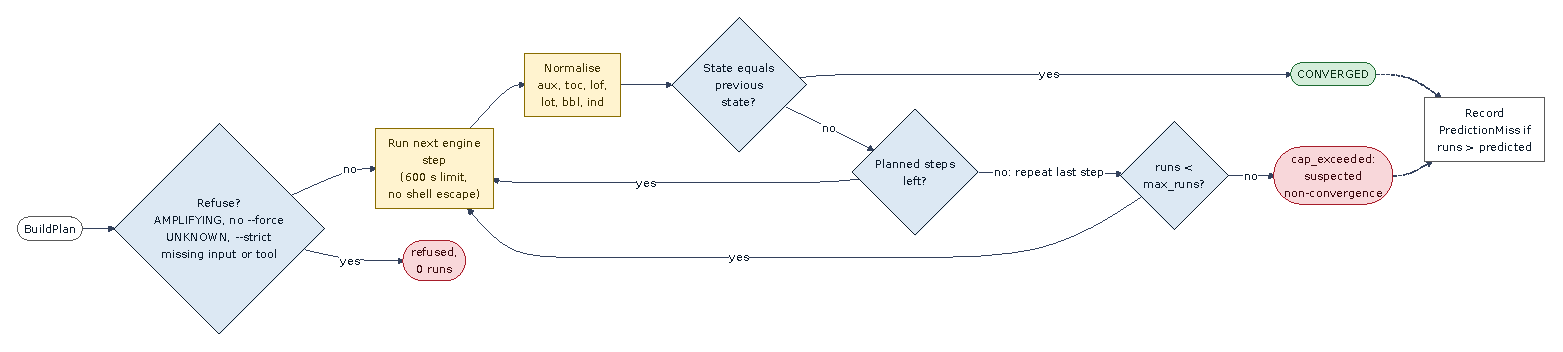
\includegraphics[width=\textwidth]{runtime.pdf}
\caption{The verification loop of \texttt{auxflow run}. A plan that ran to its last step is checked, and extended only while the auxiliary state still changes.}
\label{fig:runtime}
\end{figure*}

%% ---------------------------------------------------------------------------------------------
\section{Worked Example}
\label{sec:example}

Figure~\ref{fig:b08} shows document \texttt{b08} of our corpus.
It is Gaspar's mechanism M1 in a compact form.
\begin{small}
\begin{verbatim}
 5 \whiledo{\value{generatedpage}
 6           <\pageref{end:generated}}{%
 7   \stepcounter{generatedpage}%
 8   Record sheet occupies its own page.
 9   \newpage }
10 End of the record.\label{end:generated}
\end{verbatim}
\end{small}
The loop reads the page of the label.
Each pass of the loop emits one page.
The label sits after the loop, so the loop changes the page that it reads.

\begin{figure*}[t]
\centering
\begin{minipage}[b]{0.47\textwidth}
\centering
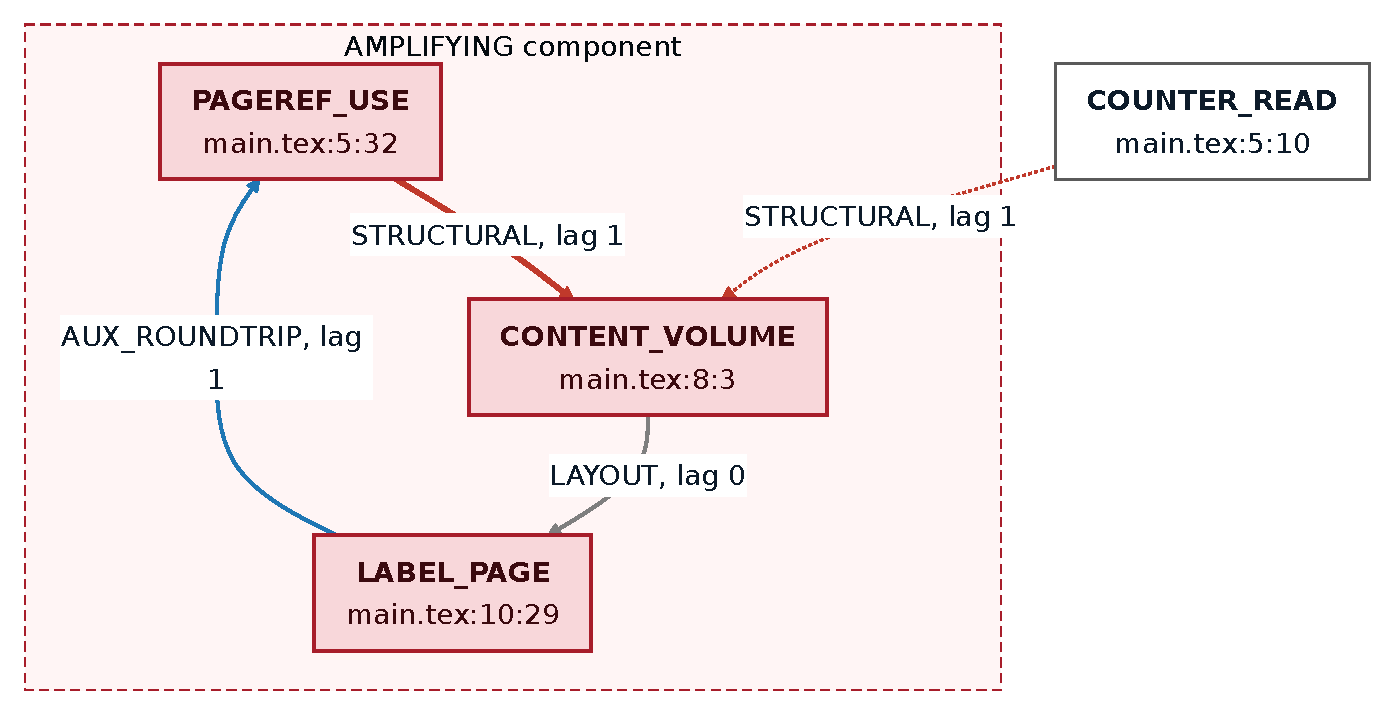
\includegraphics[width=0.78\linewidth]{arg-b08.pdf}
\end{minipage}\hfill
\begin{minipage}[b]{0.50\textwidth}
\centering
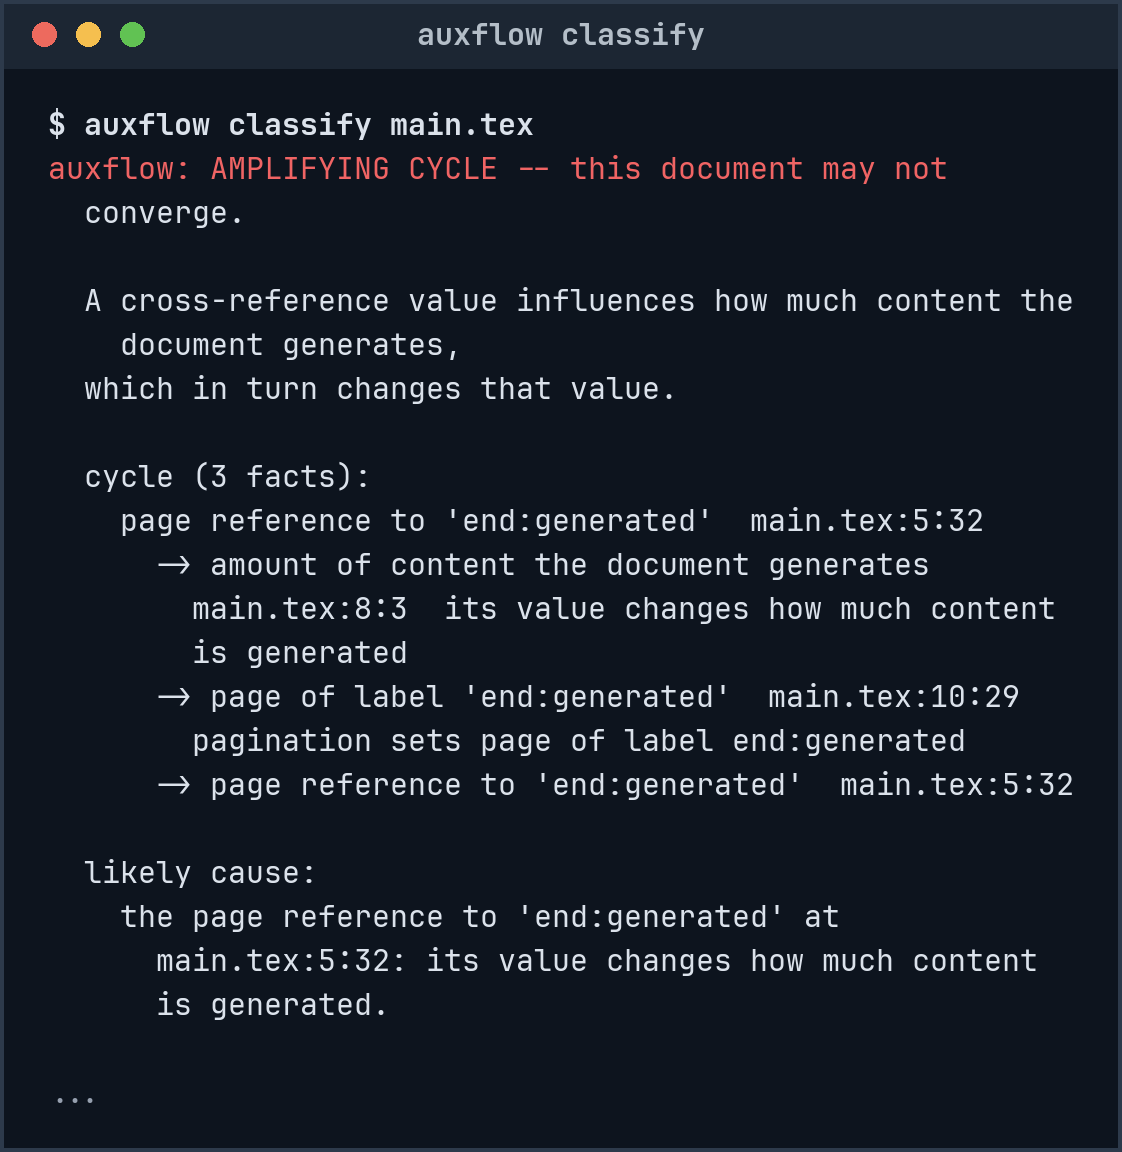
\includegraphics[width=0.98\linewidth]{shot-amplifying.png}
\end{minipage}
\caption{Document \texttt{b08}. Left: its ARG. The edge from the page reference to \textsc{content\_volume} is added by the taint analysis. Right: the report of \texttt{auxflow classify}, cut at 21 lines. Both come from the same source location data.}
\label{fig:b08}
\end{figure*}

The taint analysis seeds the page reference at line 5, because the loop condition reads it.
The analysis adds a structural edge to the volume of content.
The layout edge then reaches the label page, and the round trip returns to the reference.
The three facts form one component with an internal structural edge, so the document is amplifying.
AuxFlow reports this without an engine run.
The report names the chain and the three source locations.

With \texttt{--force}, AuxFlow runs the document under the cap.
The page count grows by one on every run, and the verifier stops at run six with \cls{cap\_exceeded}.
Figure~\ref{fig:shots} shows this run and the report for an UNKNOWN document.

\begin{figure*}[t]
\centering
\begin{minipage}[t]{0.49\textwidth}
\centering
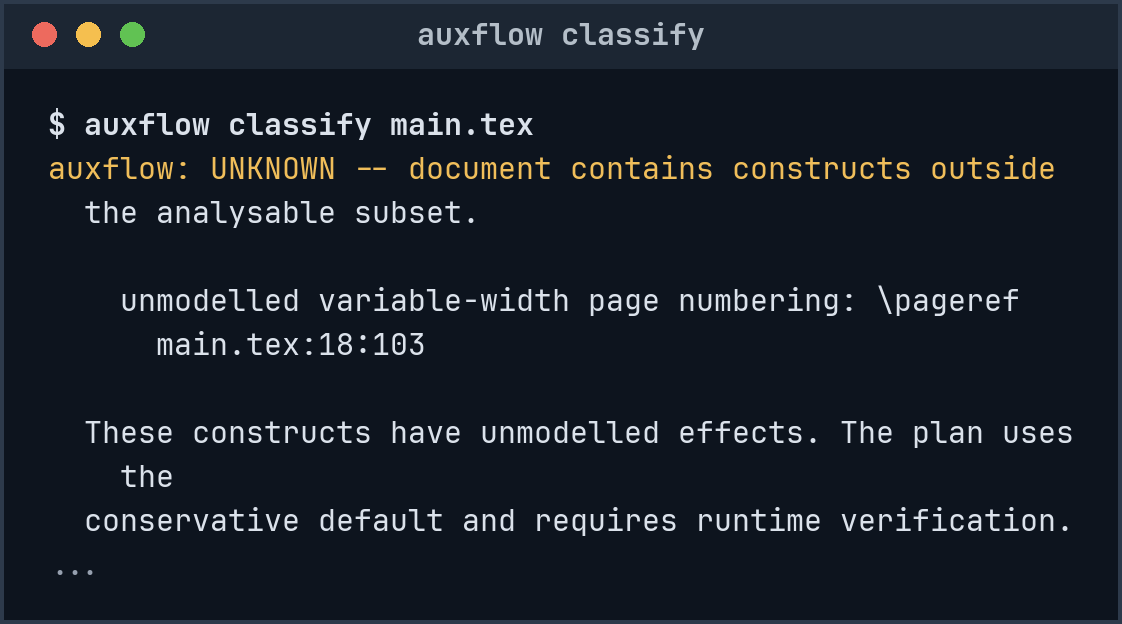
\includegraphics[width=0.98\linewidth]{shot-unknown.png}
\end{minipage}\hfill
\begin{minipage}[t]{0.49\textwidth}
\centering
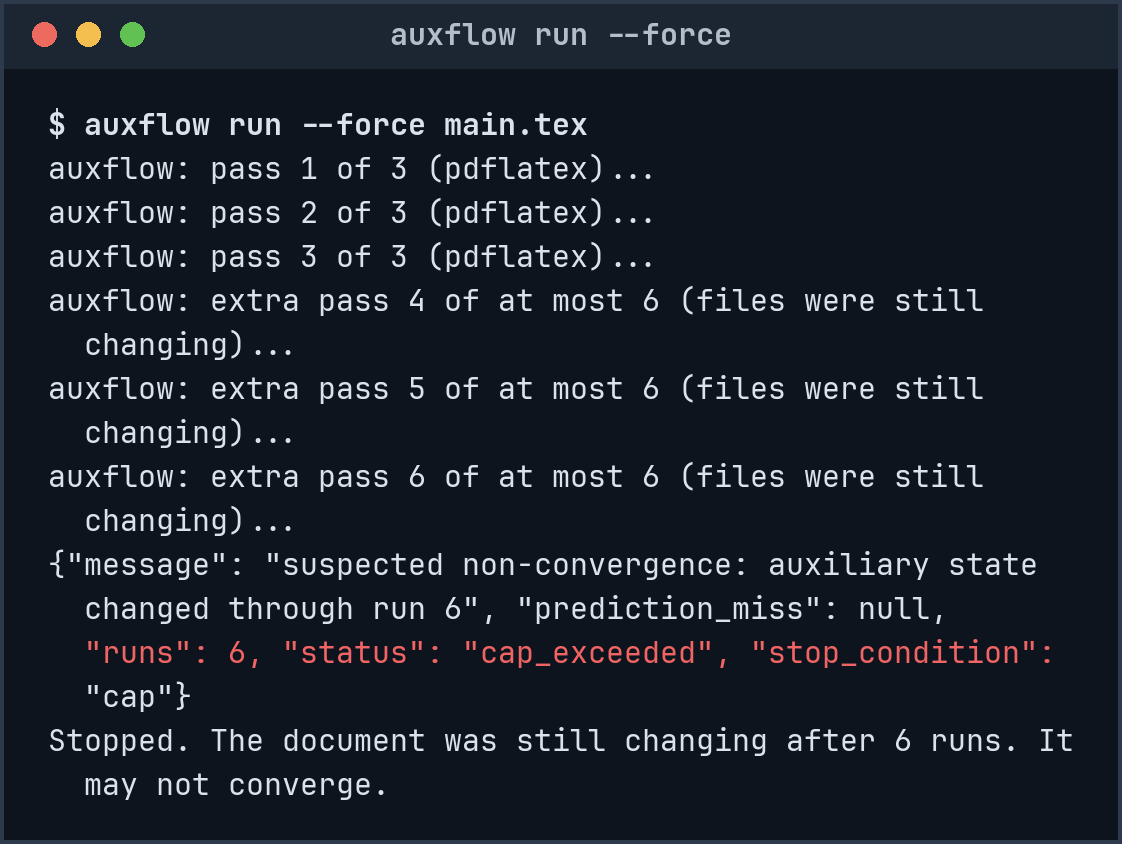
\includegraphics[width=0.98\linewidth]{shot-run.png}
\end{minipage}
\caption{Left: \texttt{auxflow classify} on \texttt{b11}. Right: \texttt{auxflow run --force} on \texttt{b08}. The run stops at the cap of six runs.}
\label{fig:shots}
\end{figure*}

%% ---------------------------------------------------------------------------------------------
\section{Evaluation}
\label{sec:eval}

\subsection{Questions and design}

We ask four questions.
\begin{description}
\item[RQ1] Does the classifier separate the modeled mechanisms, and which mechanisms does it miss?
\item[RQ2] Is the bound $N$ at least the measured run count $N^{*}$ for every certified document?
\item[RQ3] How do the stopping tests differ in verdict and in engine runs?
\item[RQ4] What does the analysis cost?
\end{description}

Figure~\ref{fig:eval} shows the setup.
The corpus has \NDocs{} documents.
Each document isolates one mechanism.
We wrote the expected classification of each document before we wrote the analyzer.
We included three documents that the analyzer was expected to misjudge, so that a predicted miss counts as a result and not as a defect.

\begin{figure*}[t]
\centering
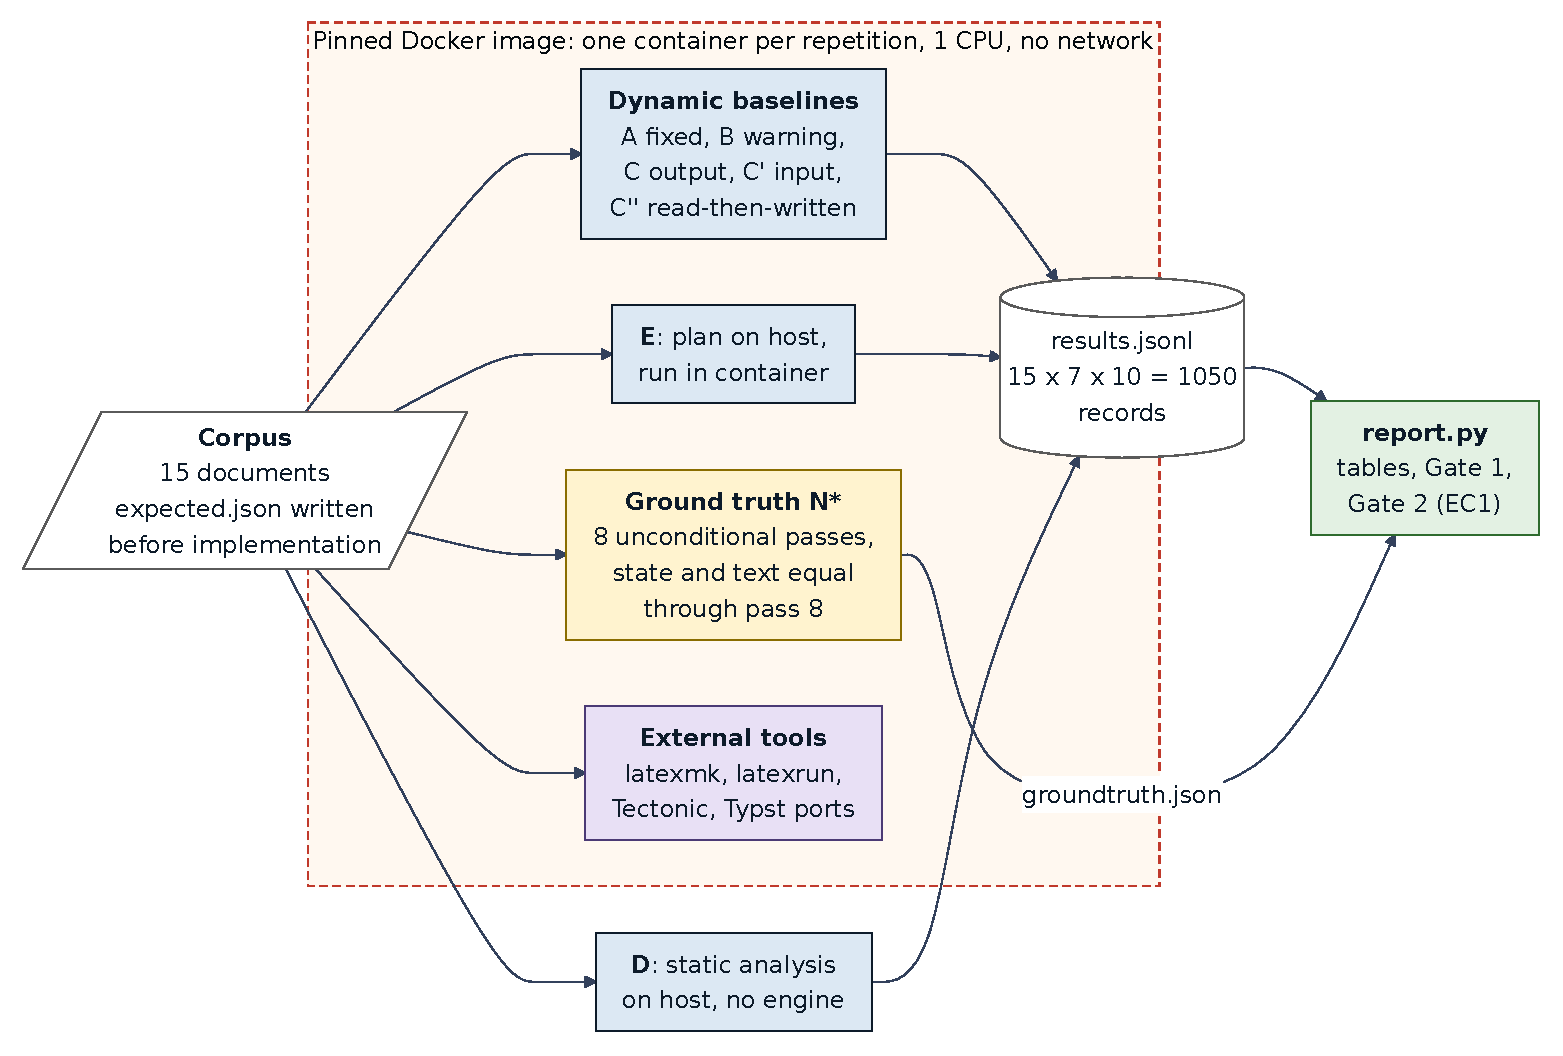
\includegraphics[width=0.86\textwidth]{evaluation.pdf}
\caption{Evaluation design. Baselines A to E run inside a pinned container. Baseline D runs on the host and never starts an engine.}
\label{fig:eval}
\end{figure*}

The baselines are:
A, a fixed schedule of three runs;
B, the kernel rerun warning;
C, comparison of the state after consecutive runs (the test of \texttt{latexmk});
C$'$, comparison of the engine inputs (\texttt{latexrun});
C$''$, comparison of files that were read and then rewritten in one run (Tectonic);
D, AuxFlow static analysis alone;
and E, the AuxFlow plan with runtime verification.
Every dynamic baseline stops at eight runs.
For E, an UNKNOWN document is refused, as under \texttt{auxflow run --strict}.

\textbf{Ground truth.}
We run the engine eight times without a stopping rule.
$N^{*}$ is the smallest $k<8$ such that the auxiliary state and the text layer from every run $k$ to $8$ equal those of run $8$.
This definition needs the ``every run'' clause.
Without it, a document that alternates between two states matches at every even $k$ and gets a false finite $N^{*}$.
We found this problem in the first measurement and corrected the harness.
A document without such a $k$ is \emph{divergent} or \emph{oscillating}.

\textbf{Environment.}
One container per repetition, one CPU, no network, and fixed \texttt{SOURCE\_DATE\_EPOCH}.
The image has TeX Live 2022 from Debian bookworm, latexmk 4.79, latexrun, Tectonic 0.15.0, and Typst 0.11.0.
Its digest begins with \texttt{\ImageDigest}.
We ran ten repetitions for each document and baseline.
All repetitions agree for every cell of Table~\ref{tab:exec}, except where the text says otherwise.
We report medians, and we report no corpus-wide mean.

\begin{table}[t]
\caption{Corpus. $N^{*}$ is the measured run count (div.: divergent, osc.: oscillating). ``Before'' is the classification in the first run. ``Now'' is the classification of the current analyzer. Bold marks a change. $N$ is the predicted run count.}
\label{tab:corpus}
\centering
\footnotesize
\begin{tabular}{@{}llrllr@{}}
\toprule
ID & Mechanism & $N^{*}$ & Before & Now & $N$ \\
\midrule
b01 & no auxiliary facts & 1 & CERT & CERT & 1 \\
b02 & backward \texttt{\char92 ref} & 2 & CERT & CERT & 2 \\
b03 & forward \texttt{\char92 ref} & 2 & CERT & CERT & 2 \\
b04 & TOC, then \texttt{\char92 pageref} & 2 & CERT & CERT & 3 \\
b05 & table of contents & 3 & CERT & CERT & 3 \\
b06 & TOC, BibTeX, \texttt{\char92 pageref} & 3 & CERT & CERT & 4 \\
b07 & M7 footnote feedback & 2 & UNK & UNK & -- \\
b08 & M1 page-bounded loop & div. & AMPL & AMPL & -- \\
b09 & multi-chapter thesis & 3 & CERT & CERT & 4 \\
b10 & M8 random auxiliary record & div. & UNK & UNK & -- \\
b11 & M3 numeral width & osc. & CERT & \textbf{UNK} & -- \\
b12 & M4 float, Roman numerals & osc. & CERT & \textbf{UNK} & -- \\
b13 & M6 \texttt{varioref} text & osc. & CERT & \textbf{UNK} & -- \\
b14 & M2 page-conditioned size & osc. & AMPL & AMPL & -- \\
b15 & M5 \texttt{ibid} citation style & 3 & UNK & UNK & --%
\\
\bottomrule
\end{tabular}
\end{table}

\subsection{Classification and the bound (RQ1, RQ2)}

Table~\ref{tab:corpus} shows the result.
Document \texttt{b08} is amplifying.
Document \texttt{b05}, the table of contents, is certified and is not amplifying.
These two checks guard against a vacuous analysis, and both pass.
Document \texttt{b14} is amplifying too.
It is a true positive that comes from over-approximation.
Nothing in \texttt{b14} changes the quantity of content, only its size.
Typst compiles the ported document without an error, which shows that the verdict is a conservative one.

All \NCertified{} certified documents satisfy $N\ge N^{*}$.
The bound is exact for \BoundTight{} documents and larger by one for \BoundOverOne{}.
It is never too small (\BoundUnder{} cases).
A larger bound is expected, because the analysis does not claim a minimum.

The analyzer flags all \NNonconv{} non-convergent documents.
It labels two amplifying and four UNKNOWN.
It certifies none of them.
This result differs from the first measurement, and Section~\ref{sec:guard} explains why.

\subsection{Stopping tests (RQ3)}

Table~\ref{tab:exec} and Fig.~\ref{fig:exec} give the engine runs until each test reached a verdict.
Table~\ref{tab:verdict} counts the verdicts.

\begin{table}[t]
\caption{Engine runs until a verdict (median of ten). $\dagger$: the baseline accepted the document as converged although the output was stale or the document never settles. cap: the baseline stopped at its limit. ref.: AuxFlow refused to run.}
\label{tab:exec}
\centering
\footnotesize
\setlength{\tabcolsep}{4pt}
\begin{tabular}{@{}lrrrrrrr@{}}
\toprule
ID & $N^{*}$ & A & B & C & C$'$ & C$''$ & E \\
\midrule
b01 & 1 & 3 & 1 & 2 & 2 & 2 & 2 \\
b02 & 2 & 3 & 2 & 2 & 2 & 2 & 2 \\
b03 & 2 & 3 & 2 & 2 & 2 & 2 & 2 \\
b04 & 2 & 3 & 2 & 2 & 2 & 2 & 2 \\
b05 & 3 & 3 & 1$^\dagger$ & 3 & 3 & 3 & 3 \\
b06 & 3 & 3 & 3 & 3 & 3 & 3 & 3 \\
b07 & 2 & 3 & 2 & 2 & 2 & 2 & ref. \\
b08 & div. & 3$^\dagger$ & cap & cap & cap & cap & ref. \\
b09 & 3 & 3 & 3 & 3 & 3 & 3 & 3 \\
b10 & div. & 3$^\dagger$ & 1$^\dagger$ & cap & cap & cap & ref. \\
b11 & osc. & 3$^\dagger$ & cap & cap & cap & cap & ref. \\
b12 & osc. & 3$^\dagger$ & cap & cap & cap & cap & ref. \\
b13 & osc. & 3$^\dagger$ & cap & cap & cap & cap & ref. \\
b14 & osc. & 3$^\dagger$ & cap & cap & cap & cap & ref. \\
b15 & 3 & 3 & 1$^\dagger$ & 3 & 3 & 3 & ref.%
\\
\bottomrule
\end{tabular}
\end{table}

\begin{figure*}[t]
\centering
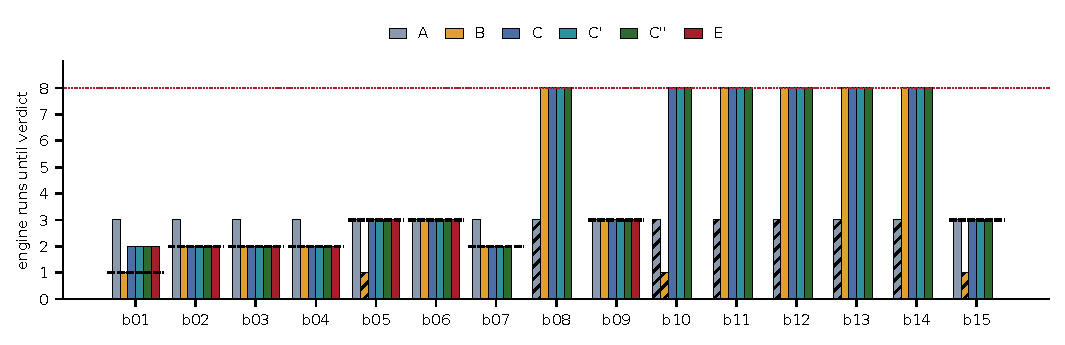
\includegraphics[width=\textwidth]{executions.pdf}
\caption{Engine runs until a verdict, by document and baseline. Dashed bars mark $N^{*}$. Hatched bars mark a wrong acceptance. Missing bars for E mark a refusal. The dotted line is the cap of eight runs.}
\label{fig:exec}
\end{figure*}

\begin{table}[t]
\caption{Verdicts over the corpus. Columns A to E are baselines. Column D is the static classification alone.}
\label{tab:verdict}
\centering
\footnotesize
\setlength{\tabcolsep}{3pt}
\begin{tabular}{@{}p{0.43\columnwidth}rrrrrrr@{}}
\toprule
 & A & B & C & C$'$ & C$''$ & E & D \\
\midrule
Correct stop, of 9 convergent documents & 9 & 7 & 9 & 9 & 9 & 7 & 7 \\
Premature stop (stale output accepted) & 0 & 2 & 0 & 0 & 0 & 0 & 0 \\
Withheld by static refusal & 0 & 0 & 0 & 0 & 0 & 2 & 2 \\
Non-convergence flagged, of 6 & 0 & 5 & 6 & 6 & 6 & 6 & 6 \\
Non-convergence accepted as converged & 6 & 1 & 0 & 0 & 0 & 0 & 0 \\
Engine runs spent on the 9 convergent documents & 27 & 17 & 22 & 22 & 22 & 17 & 0%
\\
\bottomrule
\end{tabular}
\end{table}

Four results stand out.

First, the fixed schedule A is silently wrong on every non-convergent document.
It reports three runs as done and has no way to know whether three runs were enough.

Second, the kernel warning B is unsound in both measured ways.
On \texttt{b10} it accepts a document that never settles, because a changing random value produces no reference warning.
On \texttt{b05} and \texttt{b15} it stops after one run, although $N^{*}$ is three.
The first of these is the case that the \texttt{rerunfilecheck} documentation predicts~\cite{rerunfilecheck}.

Third, the three state-comparison tests C, C$'$, and C$''$ give the same verdict on every document.
They spend \SumC{} engine runs each on the seven certified documents, and so does E.
We did not reproduce a one-run gap between output comparison and input comparison on this corpus.
We expected one from the manuals.
We did not investigate the cause, and a larger corpus may show it.

Fourth, E equals the best dynamic test in runs on the seven documents that it executes.
It spends \SumE{} runs, against \SumA{} for the fixed schedule.
It refuses eight documents before the first run: six non-convergent ones, and the two convergent ones that contain opaque constructs (\texttt{b07} and \texttt{b15}).
This is a saving of four runs over A on tiny documents, and the corpus cannot support a stronger claim.
Document \texttt{b01} needs two runs under E although $N=1$.
pdfTeX writes a page-count record to every \texttt{.aux} file, so the state is never empty, and the verifier needs a second run to see two equal states.
It logs a prediction miss on all ten repetitions.
The prediction is right, since $N^{*}=1$.
The miss comes from the confirming run that any state-comparison test needs.

\subsection{External tools (RQ3)}
\label{sec:external}

We ran \texttt{latexmk}, \texttt{latexrun}, and Tectonic on the same corpus.
This is a cross-check and not a baseline.
Every document that is not listed in Table~\ref{tab:external} converges under \texttt{latexmk} and \texttt{latexrun}.
Both tools fail on all six non-convergent documents.
This confirms that the corpus members are real non-convergence and not artifacts of the corpus.
\texttt{latexrun} also fails on \texttt{b15}, which \texttt{latexmk} accepts.
Tectonic compiles only \texttt{b01} and \texttt{b08} offline, because the other documents need files from its network bundle, and we block the network.
On \texttt{b08}, Tectonic prints that a rerun seems needed and stops at six passes.
Typst rejects our hand port of \texttt{b08} with ``loop seems to be infinite''.
This is a second independent implementation that reaches the same verdict as AuxFlow.

\begin{table}[t]
\caption{Convergence reported by external tools on the documents where at least one tool fails. n/a: Tectonic cannot compile the document offline.}
\label{tab:external}
\centering
\footnotesize
\begin{tabular}{@{}lccc@{}}
\toprule
ID & latexmk & latexrun & Tectonic \\
\midrule
b08 & no & no & cap \\
b10 & no & no & n/a \\
b11 & no & no & n/a \\
b12 & no & no & n/a \\
b13 & no & no & n/a \\
b14 & no & no & n/a \\
b15 & yes & no & n/a%
\\
\bottomrule
\end{tabular}
\end{table}

\subsection{Cost (RQ4)}

Static analysis takes \LatencyMedian{} ms at the median and \LatencyMax{} ms at most over all \NDocs{} documents.
The largest graph is \texttt{b09}, with \ThesisFacts{} facts and \ThesisEdges{} edges, at \ThesisLatency{} ms.
We report this time as overhead and do not subtract it from any run time.
We did not measure engine time per run separately, so we make no claim about the ratio of analysis time to run time.

%% ---------------------------------------------------------------------------------------------
\section{A Change After the First Measurement}
\label{sec:guard}

The first measurement ran before the guard in this section existed.
Then, documents \texttt{b11}, \texttt{b12}, and \texttt{b13} were certified.
That was the expected false negative.
Their feedback runs through the typeset width of a reference and not through a loop, so no seed reaches them.
Table~\ref{tab:corpus} shows the old and the new classification.

We then added three syntactic guards to the lowering step.
A page reference under \tex{\pagenumbering{roman}}, Roman, alph, or Alph numbering makes the document UNKNOWN, because the numeral width depends on its value.
The commands \tex{\vref} and \tex{\vpageref} make a document UNKNOWN for the same reason.
A page reference under arabic numbering is not affected, so \texttt{b03} and \texttt{b09} stay certified.
We also added a list of inert packages and commands, so that ordinary front matter does not turn a document into UNKNOWN.

This change has three consequences for how to read our results.
\begin{itemize}
\item The three expected misses are no longer misses.
The pre-registered expectation (certified) fails on these documents, and we report the gate that checks it as failed.
\item The change is post hoc.
We made it after we saw the measurement, so the corpus no longer tests the guard independently.
\item The guard matches syntax and not the mechanism.
We did not test width feedback under arabic numbering, and we expect the analysis to certify such a document.
\end{itemize}
The analysis is still incomplete, and the incompleteness is the main limit of the method.

%% ---------------------------------------------------------------------------------------------
\section{Threats to Validity and Limitations}

\textbf{Corpus size.}
The corpus has fifteen documents, and most are synthetic.
Only \texttt{b09} resembles a real document.
Every statement about run counts applies to this corpus.

\textbf{Author bias.}
The same person wrote the corpus, the expectations, and the analyzer.
The expectations came first, and they are in the repository.
This reduces the risk but does not remove it.

\textbf{Assumption A2.}
The model assumes that resolving a reference does not change pagination.
That assumption is false.
Replacing \texttt{??} with a number can change a line break.
Without the assumption, every document with a reference is one component.
With it, the analysis is unsound for the extent-driven class.
We chose the second option.
We measure the unsoundness and do not claim to remove it.

\textbf{Divergence and oscillation.}
Our amplifying label covers two different failures.
A monotone loop violates the finite-height condition.
A page-conditioned size alternates, which violates monotonicity.
A split of the label would follow the theory, but the second class is mostly invisible to the analysis.

\textbf{Benign cycles.}
The bound for a benign cycle is a heuristic, and the corpus has no benign cyclic member.
We treat it as unvalidated.

\textbf{Platform.}
The container holds TeX Live 2022.
The host in our screenshots holds a newer release.
Run counts may differ with other releases.
We found one measurement error of this kind in our own process: leftover auxiliary files in a corpus directory made three baselines stop early on \texttt{b05}.
We removed those records and ran them again.

\textbf{Scope.}
AuxFlow analyzes a declared subset.
It does not implement TeX, does not expand macros, and does not claim a minimum run count.
A cycle in the ARG is not sufficient for non-convergence, and its absence is not sufficient for convergence.

%% ---------------------------------------------------------------------------------------------
\section{Conclusion}

A document can change the graph that decides its own run count.
For that reason, classical pass numbering does not apply to every LaTeX document.
AuxFlow tests whether it applies.
On our corpus, the test flagged every non-convergent document before the first engine run and bounded every certified document correctly.
It also ran in about one millisecond.

The evidence has clear limits.
The corpus is small.
The width guard is syntactic and was added after the first measurement.
The analysis cannot see most extent-driven feedback.
The next steps are a larger corpus of real documents, a test for width feedback that does not depend on syntax, and a split of the amplifying label into divergent and oscillating cases.

\section*{Availability}

The source, corpus, harness, and result files are in the AuxFlow repository~\cite{auxflow}.
Run \texttt{python paper/make\_results.py} to regenerate every table in this paper from the result files.

\bibliographystyle{IEEEtran}
\bibliography{refs}

\end{document}
